\documentclass[12pt, a4]{article}
\usepackage{graphicx}
\usepackage[T1]{fontenc}
\usepackage[utf8]{inputenc}
\usepackage{linguex}
\usepackage{subcaption}
\def\refdash{}
\def\firstrefdash{}
\usepackage{natbib}
\usepackage{times}
%\usepackage{libertinus}

% cut pages:
% pdftk degree_achievements_2020.pdf  cat 1-2 output deg-ach-2p.pdf

% uncomment according to your operating system:
% ------------------------------------------------
% ------------------------------------------------
%\usepackage{mathptmx} %% use fitting times fonts also in formulas
%\usepackage{enumerate}
\usepackage{multirow}
\usepackage[dvipsnames,table,xcdraw]{xcolor}
\usepackage{amsmath,amsthm, amssymb, latexsym}
\usepackage{fancybox}
%\usepackage{calc}
%\usepackage{mathrsfs}
%\usepackage{multirow}
%\usepackage{multicol}
\usepackage[margin=2.5cm]{geometry} %[margin=0.5in]
%\usepackage{gb4e,qtree}
%\noautomath
\usepackage{stmaryrd}
%\usepackage{pifont}
\usepackage[normalem]{ulem}
\usepackage{hyperref}

\usepackage{wrapfig}
\hyphenation{im-pli-ca-ture}
% \newcommand{\change}[2]{\textcolor{gray}{{\scriptsize\sout{#1}}\-}\textcolor{blue}{#2}}
 \newcommand{\change}[2]{\textcolor{black}{#2}}


\def\sk#1{\setbox1\hbox{#1}\rule[.5ex]{\wd1}{.4pt}\hspace*{-\wd1}{\box1}}
%\newcommand{\lizchange}[2]{\textcolor{gray}{{\sk{#1}}\-}\textcolor{purple}{#2}}
% \newcommand{\lizchange}[2]{\textcolor{purple}{#2}}
\newcommand{\lizchange}[2]{\textcolor{black}{#2}}

\newcommand{\cond}[1]{\textsc{#1}}
\newcommand{\GeurtsNouwen}{{GN}}
\newcommand{\sem}[1]{\llbracket{#1}\rrbracket}

%\linespread{0.98}
 \newcommand{\hand}{\ding{43}}
 \pagestyle{empty}
% pdftk abstract_no-more_exp_v1.pdf cat 1-2 output abstract_no-more_exp_v2.pdf
\begin{document}

%LETOS: Abstracts should be formatted to fit within two pages (letter size or A4 paper, with 2.54 cm or 1-inch margins on all sides, 12-point Times New Roman font). An additional third page may be included exclusively for references (mandatory), large figures or tables, and lines corresponding to glosses and translations in non-English examples. Examples, whether glossed or not, should be integrated into the main text rather than collected at the end.


\begin{center}{\vspace{-2ex}{\bf  Scope Over Monotonicity: NPI Licensing with Czech “majority”}}\\
%    Mojmír Dočekal (\href{mailto:docekal@phil.muni.cz}{docekal@phil.muni.cz}), Masaryk university
\end{center}
\vspace{-1ex}
\noindent \textbf{Background.} Negative Polarity Items (NPIs) are classically analyzed as markers of downward inferences (DIs; Ladusaw \citeyear{ladusaw1979polarity}), yet experimental evidence for this link remains mixed. While Szabolcsi et al. (\citeyear{szabolcsi2008effect}) found no correlation between DIs and NPI licensing, later studies suggested a relationship based on subjective judgments (Chemla et al. \citeyear{chemla2011modularity}; Denić et al. \citeyear{denic2021influence}). Barker (\citeyear{barker2018negative}) offers an alternative: NPIs signal \textit{narrow scope} with respect to their licensor rather than monotonicity per se. \citet{docekal-chumchalova-sub30} on Czech double licensing (DL) environments provided further evidence for this dissociation: NPI licensing proved domain-sensitive (following Homer \citeyear{homer2021domains}'s locality constraints), yet inference patterns remained uniformly upward-entailing. Crucially, however, DL environments still involve \textit{monotonic} operators (negation, \textit{doubt}) with complex scope interactions; they do not constitute a genuinely non-monotonic licensing context. This leaves open whether NPIs can appear in \textit{empirically non-monotonic} environments (see also \citet{alexandropoulou2020there}) — a stronger test of Ladusaw's hypothesis. The quantifier \textit{většina} (“most/majority”) provides the ideal case: it is a \textit{proportional} quantifier (Barwise \& Cooper \citeyear{barwise-cooper1981}) and neither downward- nor upward-entailing with denotation $\llbracket\textit{většina}\rrbracket(A)(B)=1$ iff $|A\cap B|>|A\setminus B|$. We present a two-part experiment on Czech \textit{sebemenší} (“least”) under \textit{většina}. If NPIs are licensed in this non-monotonic environment while participants simultaneously reject both DE and UE inferences, this would provide stronger evidence against the DI–NPI link than double licensing alone — directly supporting Barker's scope-marking view.\vspace{-0.5mm}

\noindent \textbf{Experiment.} \noindent The experiment consisted of two sections: an acceptability task and an inference judgment task. We hypothesized that the PI \textit{sebemenší} in the restrictor of a \textit{most}-QP would be judged acceptable despite participants judging this environment as non-monotonic (NM). Two versions of the questionnaire were distributed: \textit{acceptability-first} and \textit{inference-first}, with N=24 and N=29 participants, respectively. The acceptability part used 9 items in a $1\times3$ factorial design. The conditions varied in the quantifier in the QP above the PI: DE \textit{all}, NM \textit{most}, and UE \textit{some}. A 1--5 Likert scale was used. We expected the conditions' mean ratings to be in descending order.\vspace{-3mm}

\exg. \textit{Všichni/Většina/Někteří} \textit{občané/-ů} \textit{se} \textit{sebemenší} \textit{vírou} \textit{v} \textit{Boha} \textit{chtěli/-a} \textit{nalezenému} \textit{dítěti} \textit{vystrojit} \textit{křest}.\label{dite}\\
all/majority/some citizens with \textit{sebe-}small faith in God wanted found.\textsc{dat} child.\textsc{dat} arrange.\textsc{inf} christening.\textsc{acc}\\
\small ‘All/Most/Some of the citizens with even the least faith in God wanted to arrange a christening for the found child.’\vspace{-3mm}

\noindent The inference task used a $2\times3$ factorial design, with 18 items. The binary factor was UE/DE entailment between the presented sentences ($circle\rightarrow shape$ or $circle\rightarrow green.circle$). The ternary factor was the presence of \textit{all/most/some} in the stimuli. As context for each question, participants were shown an image with two shape types in red and green (6 pieces each; 12 in total). The scenario, explained beforehand, stated that each such set of shapes would be placed into two boxes with opaque walls, with a window in one of them that concealed the contents' colors (see Fig \ref{tvary}). For instance, with the DE quantifier \textit{all}, the participant saw in the image that one box contained 6/6 circles. They could then infer (but not see) that all the green circles were in that box, but not that all of the shapes were. The participants were asked to answer “yes” or “no” to whether Sentence A entailed Sentence B (see the translated example in \ref{inftask}). We expected \textit{all} to obtain mostly “yes” ratings in DE scenarios, \textit{some} in UE scenarios, and \textit{most} to obtain barely any “yes” ratings overall.\vspace{-2mm}

\ex.\label{inftask}
\textit{Sentence A:} [All/Most/Some] of the circles are in the box on the right.\\
\textit{Sentence B:} [All/Most/Some] of the [shapes/green circles] are in the box on the right.\vspace{-2mm}

\noindent \textbf{Results.} Descriptive statistics are shown in Figure~\ref{fig:acceptability}: left facet for the acceptability ratings and right one for the inference responses (percentage of ``yes'' responses: upper part for the UE inference and lower part for the DE inference). We analyzed acceptability judgments using Bayesian linear mixed models and inference responses using Bayesian logistic mixed models (random intercepts for participants; maximal models failed to converge) in \textit{R} with \textit{rstanarm} (\cite{rstanarm}). Version order (acceptability-first vs. inference-first) showed no credible effect on either task ($|\hat{\beta}| < 0.3$, $\text{BF}_{01} > 4$), so we report aggregated data. The model for the acceptability part compared acceptability ratings with \textit{most} as the reference level. The posterior distribution showed decisive evidence for the expected pattern: \textit{all} was rated credibly higher than \textit{most} ($\hat{\beta}=0.43$, 95\% CrI [0.18, 0.67], $\text{BF}_{10}=5.14$) while \textit{some} was rated credibly lower than \textit{most} ($\hat{\beta}=-0.49$, 95\% CrI [-0.73, -0.24], $\text{BF}_{10}=24.6$). Both effects showed extreme evidence in favor of the alternative hypothesis (pd > 99.96\%). The second model compared inference patterns across quantifiers (\textit{all}, \textit{most}, \textit{some}) with \textit{most} as reference level and direction (DE vs. UE) with DE as reference. The posterior distribution revealed extreme evidence for the expected monotonic patterns: participants robustly endorsed DE inferences under \textit{all} ($\hat{\beta}_{\text{UE:all}}=-8.51$, 95\% CrI $[-11.57, -5.97]$, $\text{BF}_{10}=9.20\times10^5$) and UE inferences under \textit{some} ($\hat{\beta}_{\text{UE:some}}=7.09$, 95\% CrI $[5.35, 9.09]$, $\text{BF}_{10}=3.50\times10^8$). Critically, \textit{most} showed no evidence for either inference direction (UE: $\hat{\beta}=-1.30$, 95\% CrI $[-2.85, -0.04]$, $\text{BF}_{01}=1.06$), with both DE and UE inferences rejected (DE: 6.8\%, UE: 2.3\%). This dissociation confirms that \textit{most} is neither downward nor upward entailing in the inference task, despite licensing NPIs at intermediate levels ($\mu$=3.95) between \textit{all} ($\mu$=4.34) and \textit{some} ($\mu$=3.42).

\noindent \textbf{Discussion.} The results reveal a critical dissociation: the non-monotonic quantifier \textit{most} licenses NPIs at intermediate acceptability levels ($\mu=3.95$) despite showing no monotonic inference pattern in the same participants (DE: 6.8\%; UE: 2.3\%). This directly challenges Ladusaw's (1979) hypothesis that downward entailment is a synchronic licensing condition for NPIs. Unlike double licensing environments—which involve monotonic operators with complex scope interactions (Homer 2021)—\textit{most} is genuinely non-monotonic in its restrictor: participants robustly rejected \textit{both} DE and UE inferences at near-floor levels (BF$_{01}=1.06$ for direction effect), confirming its status as a non-DE/non-UE environment. This dissociation provides stronger evidence against the DI--NPI link than double licensing alone. The strength of the monotonicity effects is decisive: participants showed \textit{extreme} evidence for DE behavior under \textit{all} (BF$_{10}=9.20\times10^{5}$) and UE behavior under \textit{some} (BF$_{10}=3.5\times10^{8}$), while \textit{most} yielded no credible preference for either direction. The acceptability gradient (\textit{all}: $\mu=4.34$ > \textit{most}: $\mu=3.95$ > \textit{some}: $\mu=3.42$) mirrors this monotonicity landscape: maximal DE licensing yields the highest acceptability, genuine non-monotonicity yields intermediate acceptability, and maximal UE yields the lowest acceptability. This pattern is incompatible with Ladusaw's synchronic DE requirement but aligns with Barker's (2018) scope-marking view: NPIs signal narrow scope with respect to their licensor (i.e., they are licensed when their wide scope does not entail their narrow scope) rather than monotonicity per se. Formally, from $\exists d\,[\textit{v\v{e}t\v{s}ina}_x(F(x,d)\rightarrow P(x))]$ ("there is some degree of faith such that most people satisfy $P$") one cannot infer $\textit{v\v{e}t\v{s}ina}_x((\exists d\,F(x,d))\rightarrow P(x))$ ("most people with some degree of faith satisfy $P$")—there may be a threshold of $d$ that guarantees $P$ (first formula true, second false). Under \textit{most}, the NPI takes narrow scope within the restrictor (\textit{sebemen\v{s}\'{i} v\'{i}rou}, "least faith"), yielding an interpretable configuration despite the quantifier's non-monotonicity. The results replicate Szabolcsi et al.'s (2008) null finding while extending it to a theoretically critical case: a quantifier that is \textit{empirically} non-monotonic in inference tasks. Diachronically, NPIs may have grammaticalized in DE environments (Herburger \citeyear{Herburger-2023}), but our data show that downward inference is not synchronically necessary for licensing—only narrow scope is required.
%\end{thebibliography}

%POSLEDNÍ STRANA: 1. 6 řádků za glosy na straně 1, 2. figury, 3. literatura
%koukám, jak vypadá automatický seznam referencí, proto ta úprava citací, ale to tam stejně nenarvem.

\begin{figure}[h]
\centering
\begin{minipage}{0.48\textwidth}
\centering
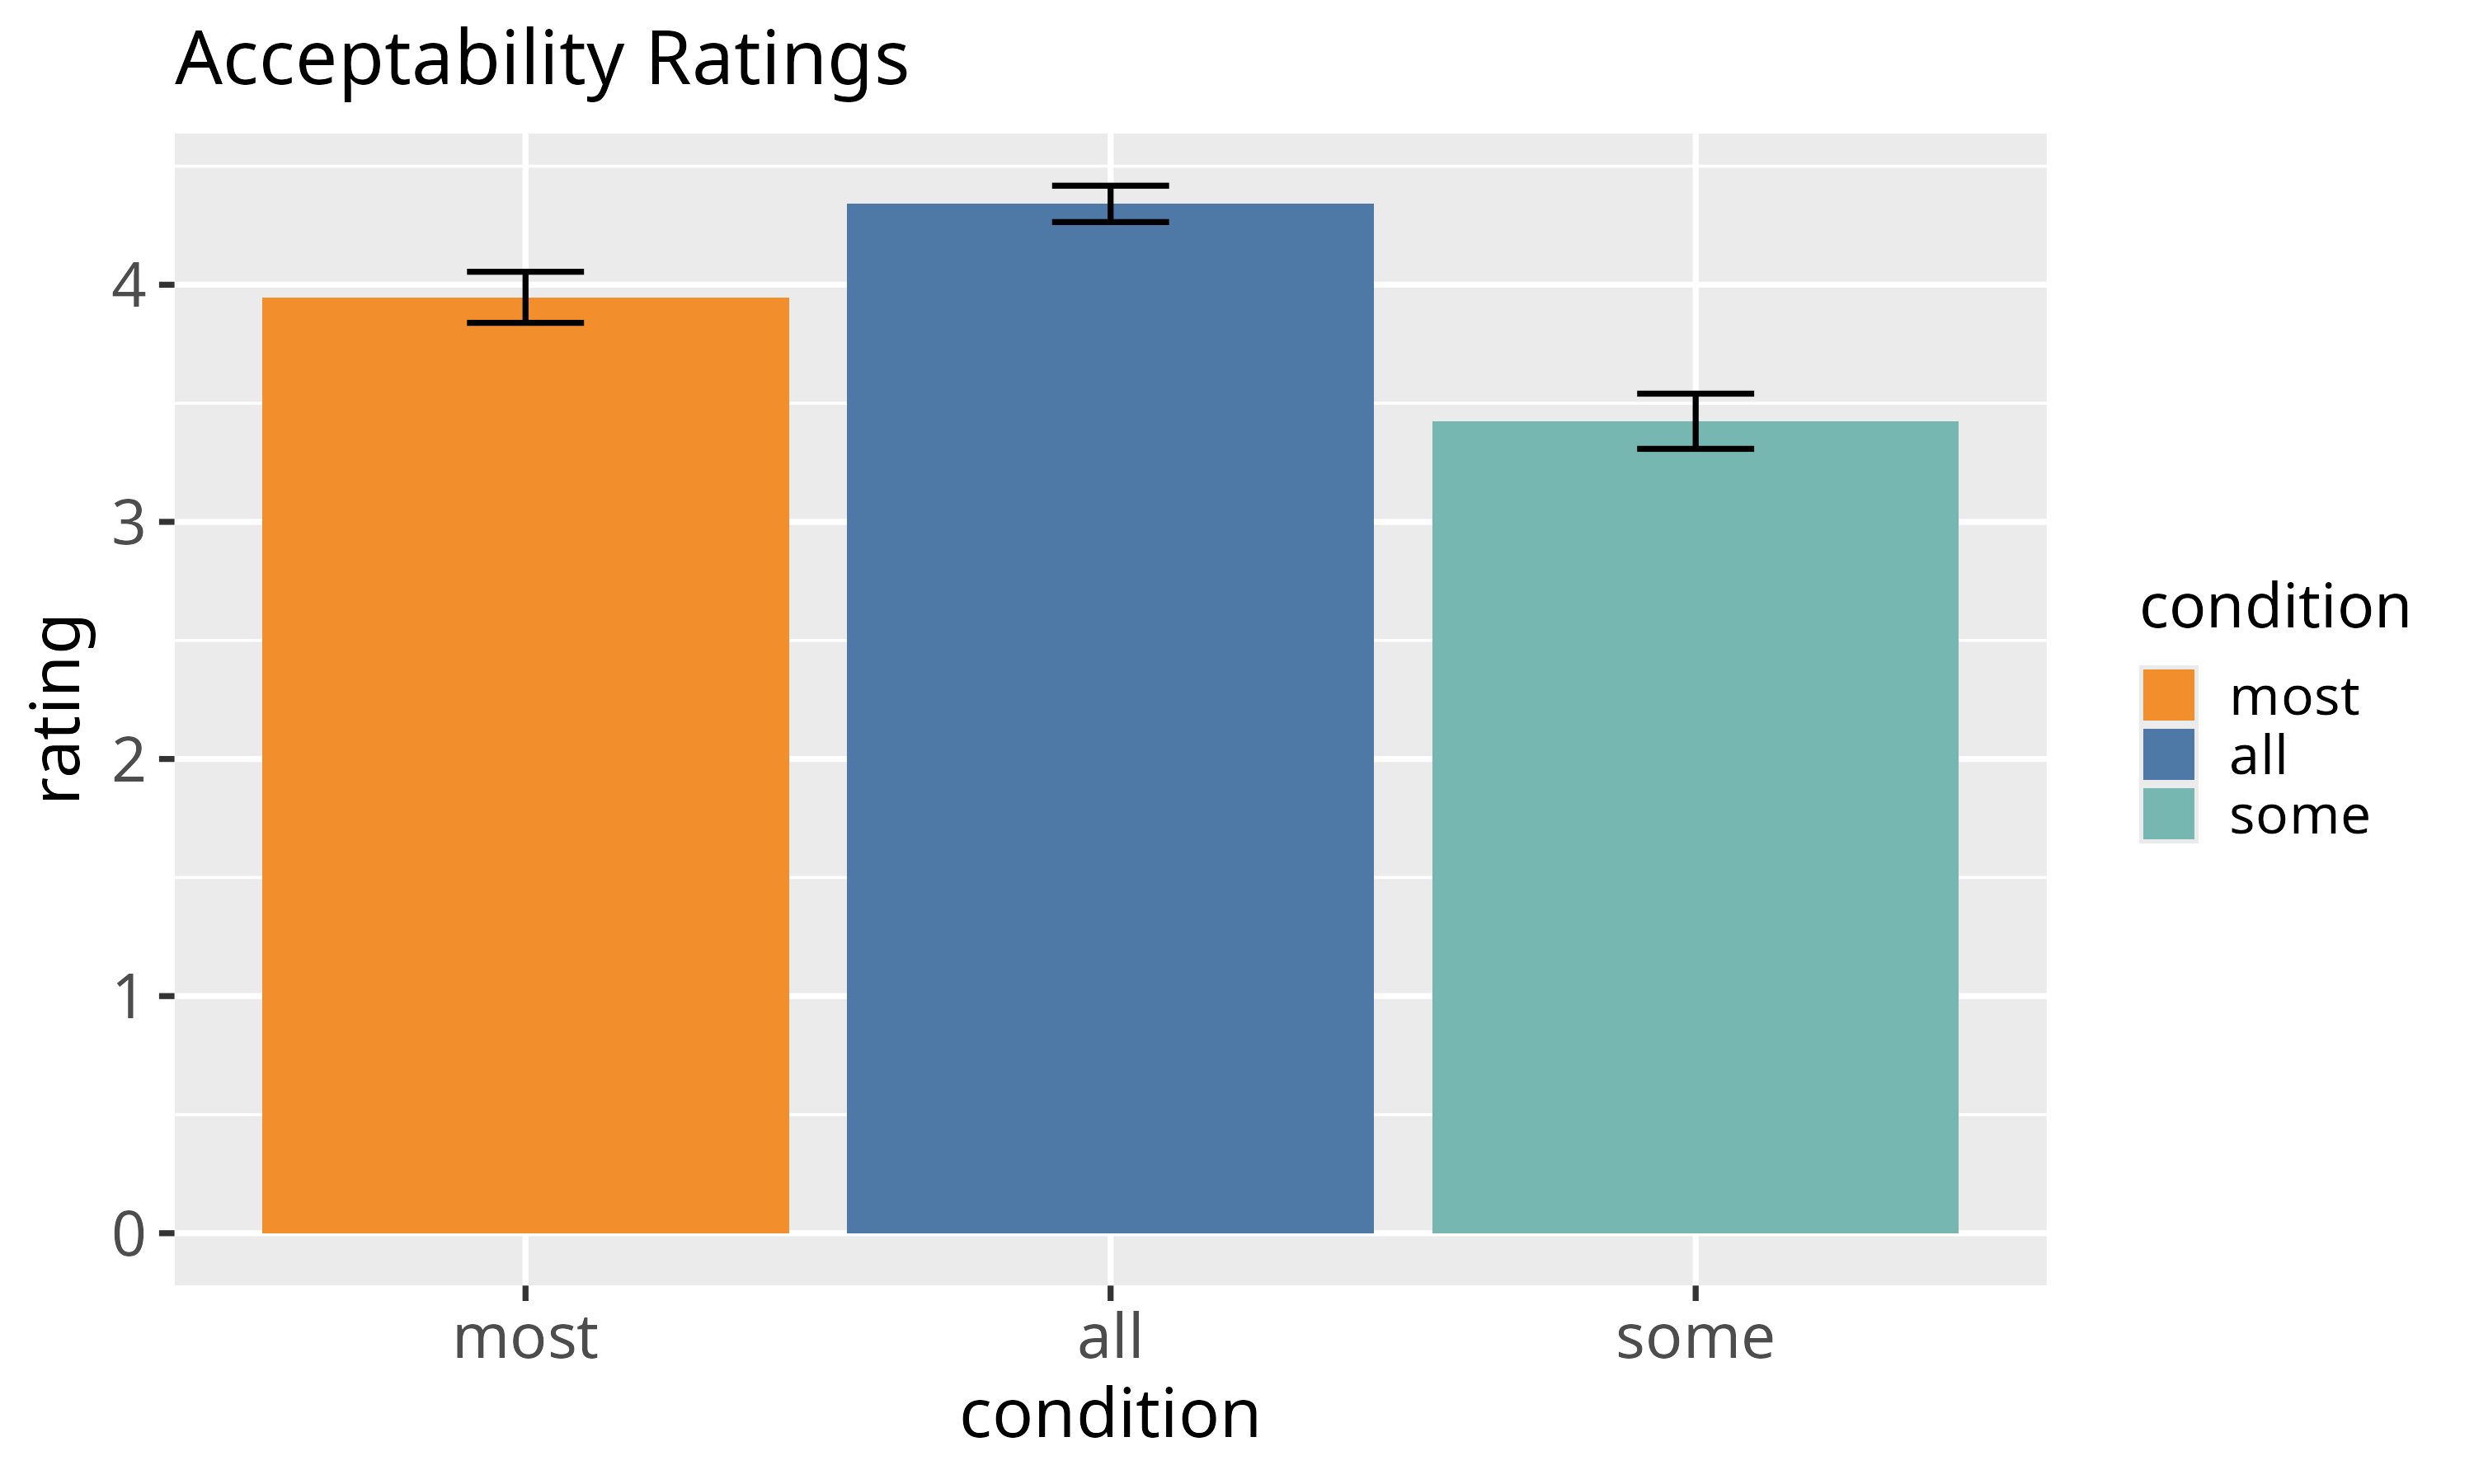
\includegraphics[width=\textwidth]{acceptability_ratings_errorbar.png}
\end{minipage}\hfill
\begin{minipage}{0.48\textwidth}
\centering
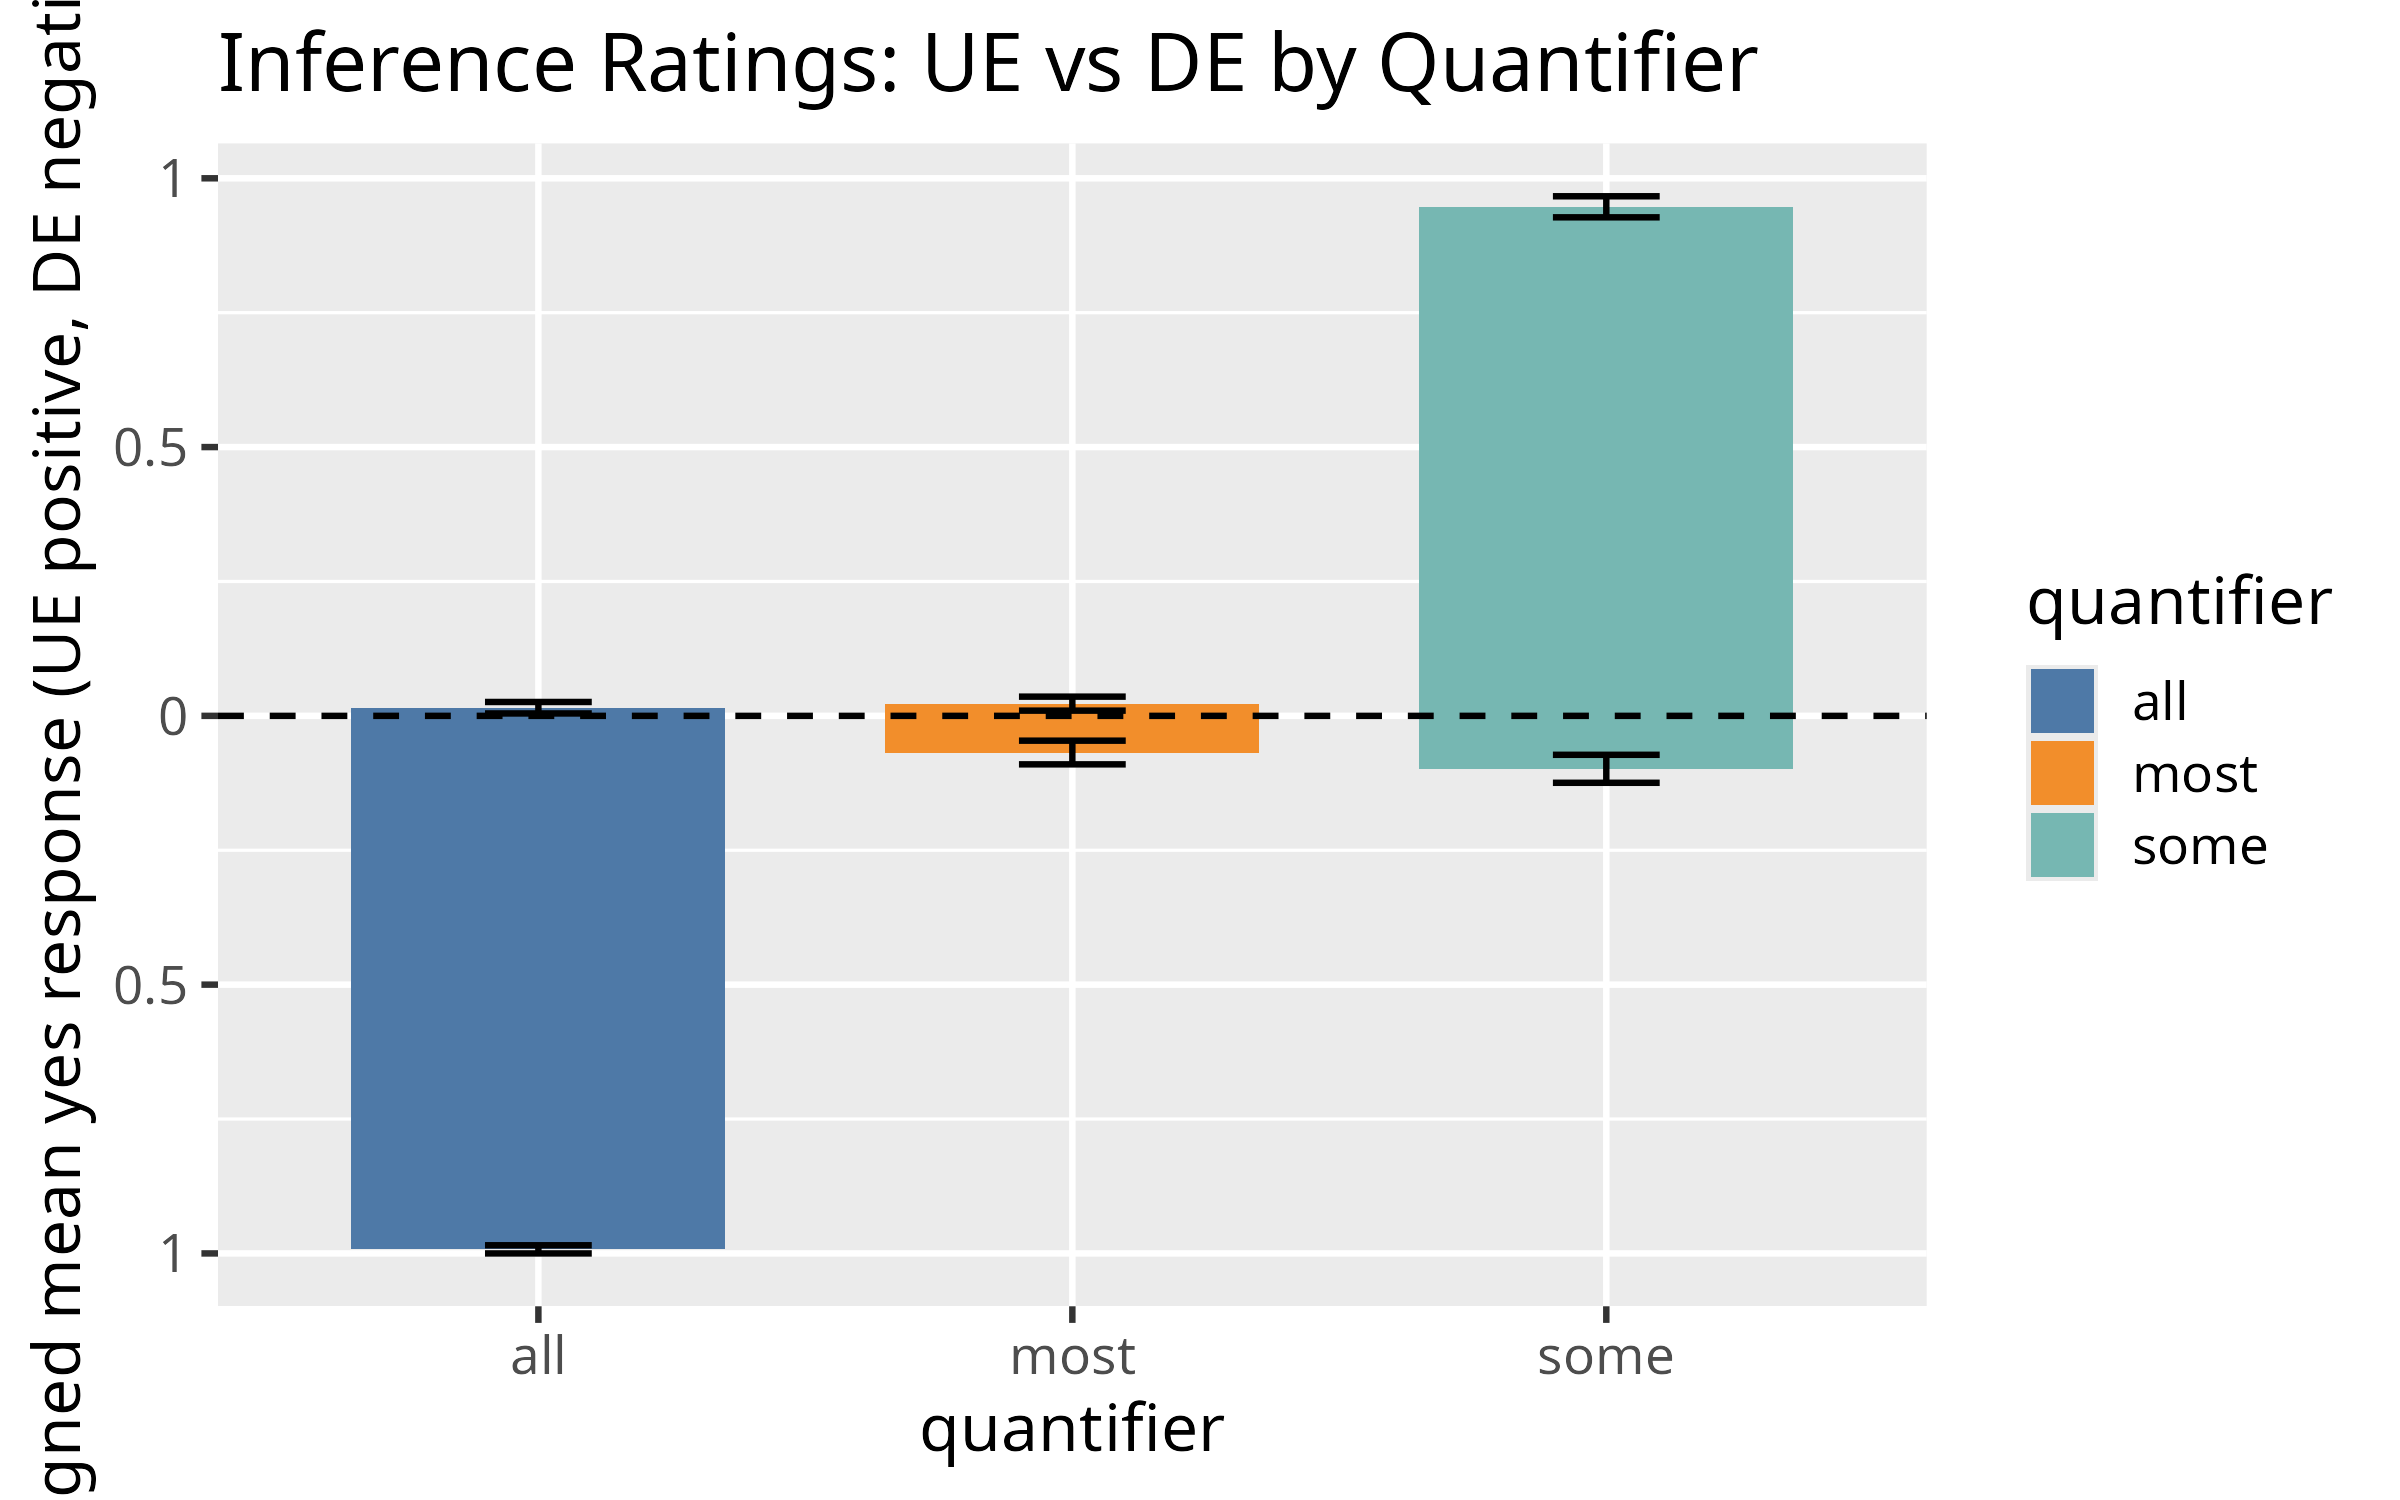
\includegraphics[width=\textwidth]{inference_ue_de_signed.png}
\end{minipage}
\caption{Acceptability ratings with error bars (left) and inference responses (right)}
\label{fig:acceptability}
\end{figure}

\vspace{-10pt}\begin{figure}[htbp]
\centering
\begin{subfigure}{.27\textwidth}
  \centering
  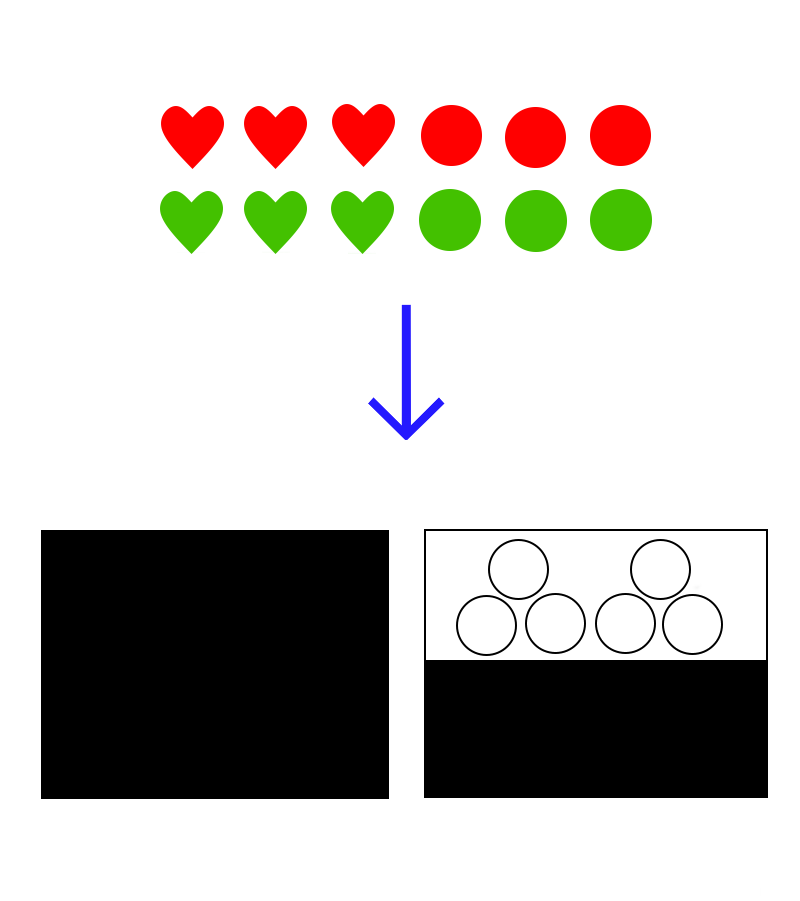
\includegraphics[width=\linewidth]{14-all.png}
\caption{ \footnotesize “all-DE” and “all-UE”} 
  \label{fig:all}
\end{subfigure}
\begin{subfigure}{.27\textwidth}
  \centering
  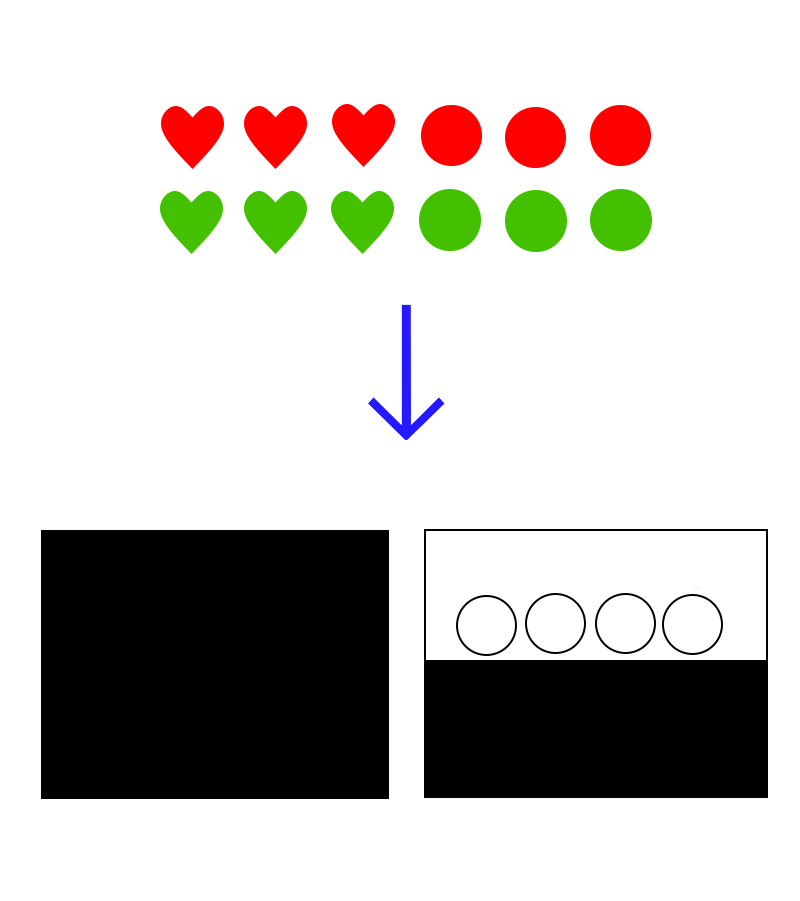
\includegraphics[width=\linewidth]{14-most.png}
  \caption{\footnotesize “most-DE” and “most-UE”}
  \label{fig:most}
\end{subfigure}
\begin{subfigure}{.27\textwidth}
  \centering
  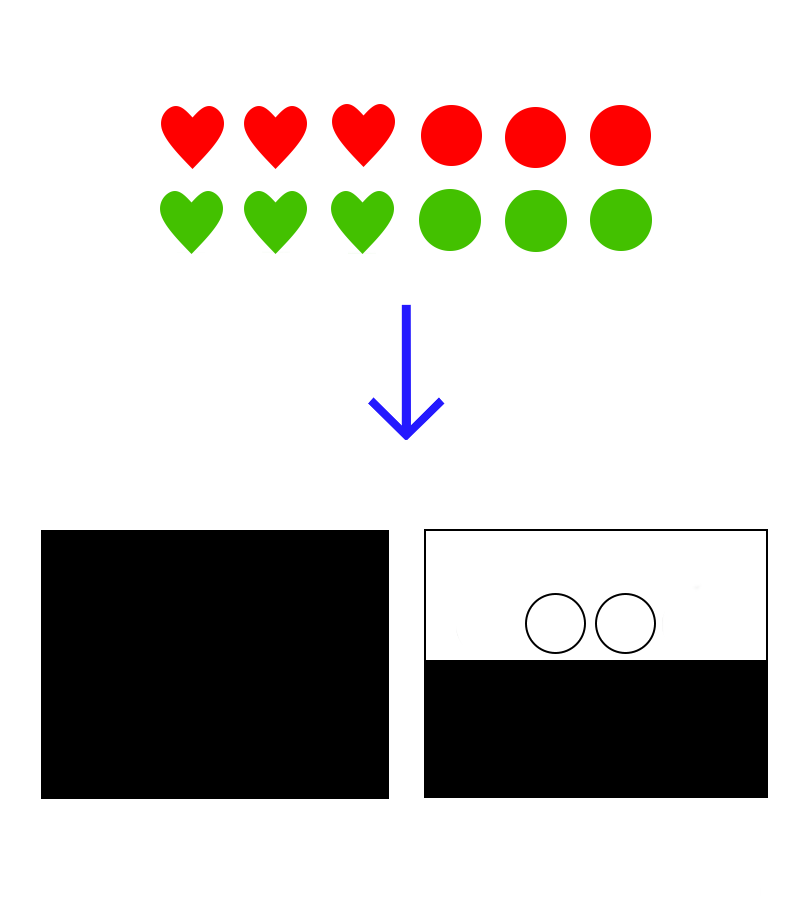
\includegraphics[width=\linewidth]{14-some.png}
  \caption{\footnotesize “some-DE” and “some-UE”}
  \label{fig:some}
\end{subfigure}
\caption{Visuals for the inference task.}\label{tvary}
\end{figure}

\vspace{+5mm}
\noindent \small \textbf{References:} Alexandropoulou, S., L. Bylinina, and R. Nouwen (2020). Is there any licensing in non-DE contexts? An experimental study. Proceedings of Sinn und Bedeutung 24(1), 35–47. $\bullet$ Barker, C. (2018). Negative polarity as scope marking. Ling. Philos. 41(5), 483–510. $\bullet$ Barwise, J. and R. Cooper (1981). Generalized quantifiers and natural language. Ling. Philos. 4(2), 159–219. $\bullet$
Brilleman, S., M. Crowther, M. Moreno-Betancur, J. Buros Novik, and R. Wolfe (2018). Joint longitudinal and time-to-event models via Stan. StanCon 2018. $\bullet$
Chemla, E., V. Homer, and D. Rothschild (2011). Modularity and intuitions in formal semantics: The case of polarity items. Ling. Philos. 34, 537–570. $\bullet$
Denić, M., V. Homer, D. Rothschild, and E. Chemla (2021). The influence of polarity items on inferential judgments. Cognition 215, 104791. $\bullet$
Dočekal, M. and L. Chumchalová (2025). NPIs, inferences and double licensing: experimental evidence. Talk at Sinn und Bedeutung 30, Goethe University Frankfurt. $\bullet$
Herburger, E. (2023). On the history of NPIs and negative concord. Canadian Journal of Linguistics 68(4), 555–589. $\bullet$ 
Homer, V. (2021). Domains of polarity items. J. Semant. 38(1), 1–48. $\bullet$ 
Ladusaw, W. A. (1979). Polarity Sensitivity as Inherent Scope Relations. Ph. D. thesis, The University of Texas, Austin. $\bullet$
Szabolcsi, A., L. Bott, and B. McElree (2008). The effect of negative polarity items on inference verification. J. Semant. 25(4), 411–450.



\newpage

\bibliographystyle{chicago}
\bibliography{bibliography_2.bib}
\end{document}
